\chapter{Introdução}

Um dos papéis da engenharia de software é fornecer métodos, modelos e técnicas para que o software atenda às necessidades dos interessados em sua construção. A utilização desse conhecimento leva a uma forma aproximadamente ideal de realizar as atividades necessárias para o desenvolvimento do software. Os resultados  gerados por atividades feitas dessa forma apresentarão um elevado grau de qualidade. Entretanto, essa forma ideal de realizar as atividades, pode exigir recursos incompatíveis com os disponíveis para o projeto. Por este motivo, as pessoas envolvidas com o projeto do software tendem a realizar essas atividades de forma que atendam às restrições de recursos e, ao mesmo tempo, estejam o mais próximas possíveis da forma ideal. Entretanto, a existência de restrições de recursos demasiadamente severas fazem com que algumas atividades tenham de ser realizadas de uma forma muito distante da ideal. Os resultados produzidos pelas atividades feitas de tal forma são chamados de dívida técnica. 

O termo dívida técnica é, na verdade, uma metafora extraída da área financeira. Realizar uma atividade de forma não ideal é como adquirir uma dívida para com a qualidade do sistema. Uma característica da dívida técnica é a de que enquanto ela não for paga, ou seja, enquanto a atividade não seja refeita produzindo resultados mais próximos do ideal, haverá um esforço adicional para realizar futuras atividades relacionadas a dívida técnica. Esse esforço adicional é equivalente ao juros financeiros que devem ser pagos enquanto o valor emprestado não for devolvido.  

A metáfora foi usado pela primeira vez por Cunningham\cite{cunningham1993wycash}. Ele percebeu que criar porções de código, que não estivessem de acordo com as boas práticas da programação, é semelhante a contrair uma dívida para com o sistema. Assim como na área financeira, essas dívidas causam o pagamento de juros. Esses juros são todas as dificuldades adicionais necessárias para manipular as porções de código feita de forma incompatível com as boas práticas. Embora a existência de dívidas técnicas traga consequências ruins para a evolução do software, nem sempre elas são algo totalmente negativo. Muitas vezes, adquirir uma dívida técnica é a opção mais correta para que haja um ganho de velocidade e não se perca uma oportunidade de negócio por exemplo. 

Apesar de poder ser um artifício estratégico viável, a aquisição de dívidas técnicas não pode ser algo feito descontroladamente. Por isso, é necessário que haja um gerenciamento para mantê-la em patamares aceitáveis.  Caso o seu nível atinja um patamar muito alto, é possível que o juros causado por ela inviabilize todo o processo de desenvolvimento e evolução do software. Esta inviabilidade se concretiza quando o esforço necessário para inserir novas funcionalidades é maior do que os benefícios trazidos por essas funcionalidades.

Neste trabalho proporemos um modelo para estimar os juros da dívida técnica em projetos de software. Esse modelo considerará os juros como a diminuição, causada pela existência da dívida técnica, da produtividade nos projetos. O modelo proposto será analisado por meio de um estudo de caso envolvendo 1814 projetos de software livre.


\section{Motivação}


  \begin{figure}[H]
  \centering
  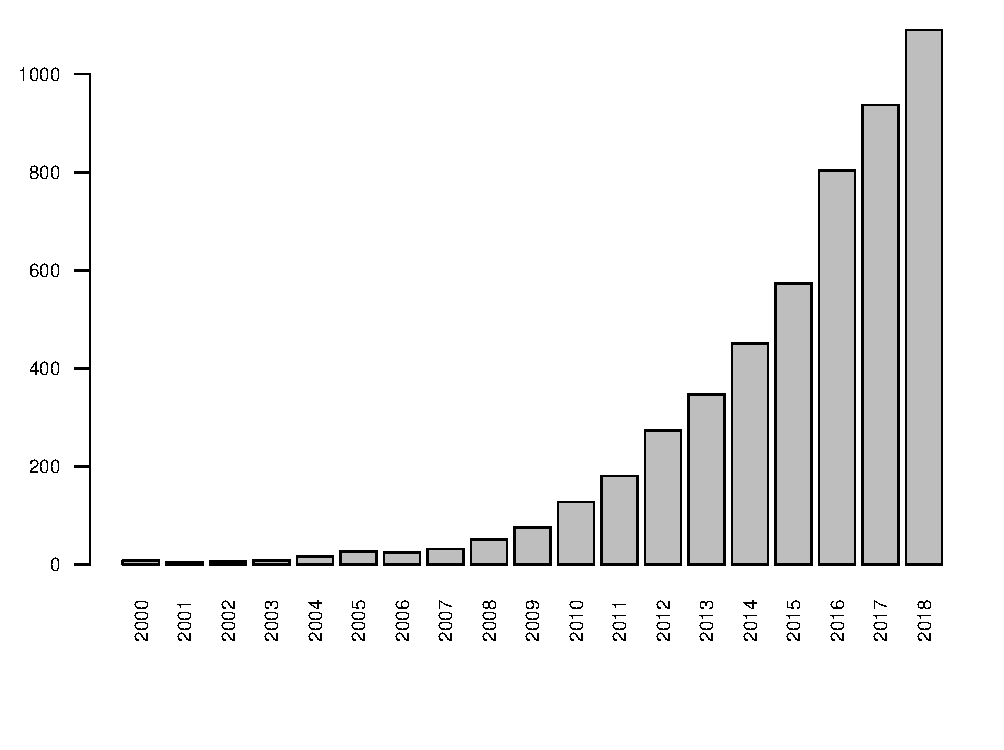
\includegraphics{capitulo_introducao/numero_citacoes.pdf} 
  \caption{Número anual de citações ao termo dívida técnica. }
  \label{fig:cap1_citacoes_td_ano} 
\end{figure}

Durante os últimos anos, como pode ser visto na Figura \ref{fig:cap1_citacoes_td_ano}, houve um acréscimo do interesse acadêmico em estudar as dívidas técnicas. Um dos assuntos estudados é o impacto dos juros da dívida nos projetos de software\cite{zazworka2011investigating,power2013understanding}. À medida que a dívida técnica é acumulada inadvertidamente,  cada vez mais atividades são realizadas apenas para estabilizar o software em vez de adicionar funcionalidades e melhorias. Em certos casos, inclusive, é cogitado o descarte do software atual a fim de que uma nova versão seja produzida do início \cite{sterling2010managing}. Uma das dificuldades para a realização do gerenciamento da dívida técnica é a falta de técnicas que auxiliem a execução dessa atividade. A inexistência dessas técnicas padronizadas é causada pelo fato de que grande parte do conhecimento que existe a respeito da dívida técnica foi gerado por experiências individuais e contextuais. Dessa forma, esse conhecimento não foi devidamente validado por meio de evidências empíricas. Isso faz com que as técnicas de gerenciamento  da dívida técnica sejam escassas e não confiáveis\cite{brown2010managing}. 

O gerenciamento da dívida técnica é baseado em dois elementos:
\begin{itemize}
\item[(i)] O esforço necessário para corrigir uma dívida técnica. Essa informação é denominada como o \textbf{principal} da dívida técnica.
\item[(ii)] O esforço adicional necessário para realizar as futuras atividades de desenvolvimento, evolução e manutenção do software.  Esse esforço adicional é chamado de \textbf{juros} da dívida técnica.
\end{itemize}
 
Dentre esses dois elementos, existe uma necessidade especial em gerenciar os juros da dívida técnica. Isso acontece pois \textbf{os juros são aquilo que efetivamente influenciam negativamente os projetos de software}.  Obter estimativas a respeito dos juros é uma das principais atividades do gerenciamento da dívida técnica. O principal em si, ou seja, o esforço necessário para quitar uma dívida técnica não traz nenhuma dificuldade adicional para o projeto de software. O que faz com que seja necessário alocar recursos para quitar uma dívida técnica é o quanto os juros dessa dívida estão altos. 

Além da escassez de estudos sobre o cálculo dos juros da dívida técnica, existe uma falta ainda maior de trabalhos quantitativos. Conforme argumentado por Brown, N et al.\cite{brown2010managing}, há uma predominância na utilização de métodos qualitativos nas pesquisas a respeito da dívida técnica e isso pode levar a conclusões baseadas em intuições atraentes, porém não necessariamente corretas. Essas conclusões incorretas podem ser explicadas pela existência de dados obtidos por meio de declarações imprecisas. Essas declarações podem ser dadas pela dificuldade que as pessoas envolvidas com os projetos de software têm em assumir suas deficiências ou falhas. Por isso, Brown, N et al.\cite{brown2010managing} indica a necessidade da criação de modelos baseados em abordagens quantitativas para viabilizar a criação de rigorosas técnicas de gerenciamento da dívida técnica que possam ser aplicadas em projetos de larga escala. 


\section{Objetivos}


Os principais objetivos desta pesquisa são os seguintes:

\begin{itemize}
\item  \textbf{Propor um modelo quantitativo para estimar os juros da dívida técnica.} Devido à escassez de trabalhos quantitativos e empiricamente avaliados, acreditamos que, por meio desse modelo, haverá uma contribuição para a resolução do problema de estimação dos juros da dívida técnica. O modelo, que será proposto, é baseado na comparação da produtividade dos projetos quando eles são realizados em dois cenários diferentes: um com dívida técnica e outro sem dívida técnica. Acreditamos que haverá uma diminuição da produtividade quando há a existência de dívidas. Essa diminuição é, na verdade, os juros da dívida técnica. Conforme veremos mais à frente, outros modelos também propõem uma abordagem de estimação dos juros comparando dois cenários. Porém, nenhum deles considera a produtividade nessa comparação. 
\item  \textbf{Avaliar a utilização desse modelo em um estudo de caso envolvendo um grande número de projetos de software livre.} Apesar de poucos, existem alguns modelos para estimação dos juros. Porém, até o nosso conhecimento, nenhum deles foi submetido a uma avaliação utilizando uma quantidade signitificativa de projetos. Nesta pesquisa iremos utilizar o modelo de estimação proposto para avaliar 1814 projetos de software livre.
\item  \textbf{Permitir o aprimoramento das abordagens de gerenciamento da dívida técnica ao permitir uma estimação dos juros gerados por elas.} Por meio da aplicação do modelo de estimação, pretendemos contribuir para o gerenciamento da dívida técnica. Possibilitando que as pessoas possam ter uma estimativa de quanto juros serão pagos para as dívidas, elas poderão decidir melhor quais dívidas devem ou não ser adquiridas e principalmente qual o nível de dívida técnica é aceitável de acordo com suas necessidades. 
\end{itemize}



\section{Trabalhos relacionados aos juros da dívida técnica}
\label{modelos_existentes}

São encontradas na literatura poucas propostas de estratégias para calcular os juros da dívida técnica.  Isso fica evidente quando são analisadas alguns dos mapeamentos sistemáticos realizados na área\cite{ampatzoglou2015financial,li2015systematic,behutiye2017analyzing}. Possivelmente, uma das razões para essa escassez é a dificuldade que há em calcular e até mesmo estimar esse juros. O efeito que a dívida técnica causa no projeto de software é algo que depende de fatores que não podem ser facilmente analisados. Além disso, há uma forte influência de eventos no qual não há certeza se eles realmente ocorrerão. Um exemplo é a existência de uma dívida técnica em um trecho do código que poderá ou não ser alterado no futuro. Se ele não for, então não haverá juros já que não haverá uma dificuldade extra para alterá-lo. Prever ou estimar a ocorrência desses eventos pode ser uma tarefa impossível em algumas situações. Por isso, o problema de estimar os juros da dívida é um dos mais difíceis dentro do espectro de problemas encontrados na área do gerenciamento da dívida técnica.


Realizamos um limitado mapeamento sistemático para encontrar os trabalhos na literatura no qual foi proposta uma estratégia para estimar os juros da dívida técnica. Esse mapeamento foi realizado observando algumas das recomendações básicas feitas por Kichenham. \cite{kitchenham2004procedures}. De acordo com Petersen et al. \cite{petersen2008systematic}, um mapeamento sistemático difere de uma revisão sistemática, pois seu objetivo principal é fornecer um panorama a respeito dos  trabalhos existentes a respeito de um determinado assunto. Já na revisão sistemática, há uma preocupação em extrair informações das pesquisa primárias com o objetivo de responder questões de pesquisa específicas que não poderiam ser respondidas avaliando individualmente esse trabalhos. 

Foram encontrados sete ótimos trabalhos focados em propor soluções para o problema de estimação dos juros da dívida técnica. Organizando esses trabalhos em ordem cronológica, é possível traçar uma linha de mudanças na forma em que o problema foi sendo tratado conforme pode ser visto na Figura \ref{fig:historico_pesquisas}. Inicialmente, foram propostas soluções baseadas na ideia de que a dívida técnica era apenas um sinônimo para problema de qualidade. Conforme evidenciado por Kruchten et al. \cite{kruchten2013technical}, essa ideia foi sendo abandonada a medida que a comunidade percebeu que a dívida técnica representa uma aspecto mais amplo. Já em 2014 surgiram abordagens no qual a estimação dos juros eram realizadas por meio de ferramentas. Umas das explicações para a criação dessas ferramentas foi a vontade dos pesquisadores em tornar a metáfora dívida técnica algo mais aplicável para os desenvolvedores conforme pode ser observado no relatório a respeito da conferência realizada naquele ano\cite{falessi2014technical}.  O próximo estágio identificado foi o foco em definir teorias mais rigorosas para descrever a metáfora. Uma das formas encontradas foi recorer à métodos encontrados na literatura financeira. Por fim, podemos identificar que os trabalhos mais recentes estão voltados para analisar os juros da dívida técnica de uma forma mais contextual. Ou seja, observando mais aspectos do projeto de software que sofrem influência da dívida técnica. Esta pesquisa se encaixa nesse grupo de pesquisas já que iremos analise o impacto da dívida técnica na produtividade do projeto.


 \begin{figure}[H]
  \centering
  \frame{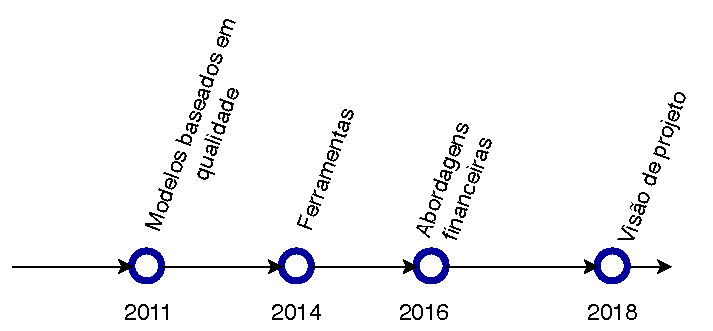
\includegraphics[trim={0cm 0cm 0cm 0cm},clip]{trabalhos_relacionados/historico_pesquisas.pdf}} 
  \caption{Quantidade de projetos por tópico do LDA.}
  \label{fig:historico_pesquisas} 
\end{figure}

  
\subsection{Mapeamento dos trabalhos relacionados}  

O mapeamento sistemático foi realizado seguindo os seguintes passos:

\begin{enumerate}
\item Foram pesquisados em banco de dados de artigos científicos trabalhos que tivessem os termos juros e dívida técnica. Não foram incluídos teses ou dissertações.
\item Inicialmente foram encontrados 5 trabalhos. Então foi realizada a aplicação de uma técnica chamada \textit{snowballing}\cite{kruchten2013technical}. Essa técnica consiste em avaliar a bibliografia dos trabalhos inicialmente encontrados e identificar outros trabalhos que possam estar relacionado ao objeto da pesquisa. Esse procedimento é feito recursivamente até que não seja encontrados novos itens. Após a aplicação dessa técnica foram encontrados mais 2 trabalhos.
\item Cada uma dos artigos foi lido e analisado por um pesquisador. Nessa análise foram extraídas as seguintes informações: Um resumo da abordagem,o método utilizado para validá-la e o ano em que foi publicada.
\end{enumerate}

A Tabela \ref{tab:resumo_trabalhos} apresenta a lista com os trabalhos encontrados.



\begin{longtable}{|m{6cm}|m{5cm}|m{2cm}|m{1cm}|}
\hline
\textbf{Título}                                                                                                              & \textbf{Resumo}             & \textbf{Método}         & \textbf{Ano}   \\  \hline
An empirical model of technical debt and interest \cite{nugroho2011empirical}                                                                  & Descrição de um framework em que os juros são calculados como a diferença entre o esforço de manutenção atual e o esforço caso o projeto estivesse com o nível máximo de qualidade. & Estudo de caso & 2011 \\ \hline
A Framework for Estimating Interest on Technical Debt by Monitoring Developer Activity Related to Code Comprehension\cite{singh2014framework} & Proposta de uma ferramenta que mede a quantidade de tempo que um desenvolvedor gasta visualizando uma classe. Essa ferramenta permite analisa a relação entre esse tempo e o nível de dívida técnica da classe.    & Experimento    & 2014 \\ \hline
Towards an open-source tool for measuring and visualizing the interest of technical debt\cite{falessi2015towards}                             & Descrição de uma ferramenta que calcula os juros utilizando a densidade dos defeitos encontrados no software.           & Estudo de caso & 2015 \\ \hline
A Financial Approach for Managing Interest in Technical Debt\cite{ampatzoglou2015financial}                                                         &   Um framework para a  estimação do ponto onde os juros pagos tornam-se maiores do que o gasto que seria necessário para eliminar a dívida técnica que os gerou.      & Exemplo        & 2016 \\ \hline
The magnificent seven: towards a systematic estimation of technical debt interest\cite{martini2017magnificent}                                    & Descrição de uma estratégia de cálculo dos juros e uma ferramenta que a implementa. A estratégia é baseada na probabilidade dos juros acontecerem e da sua severidade. A severidade é estimada por meio da avaliação de sete fatores.              & Estudo de caso & 2017 \\ \hline
Technical debt interest assessment: from issues to project \cite{martini2017technical}                                                        & Avaliação da eficácia em calcular os juros da dívida técnica como a soma dos juros dos elementos individuais do projeto. Os autores chegam a conclusão de que essa soma não é igual ao juros total do projeto.             & Estudo de caso & 2018 \\ \hline
A framework for managing interest in technical debt: an industrial validation\cite{ampatzoglou2018framework}                                        &       Versão extendida do trabalho de Ampatzoglou et al.\cite{ampatzoglou2015financial}.       & Estudo de caso & 2018 \\ \hline
\caption{Resumo dos trabalhos encontrados no mapeamento sistemático.}
\end{longtable}
\label{tab:resumo_trabalhos}


\subsection{Diferenças e semelhanças dos trabalhos relacionados e esta pesquisa}


Por meio da análise dos trabalhos encontrados no mapeamento sistemático, pudemos encontrar semelhanças e diferenças em relação a este trabalho:

\begin{itemize}

\item \textbf{Todas as propostas apresentadas comparam dois cenários: um com mais dívida técnica e outro com menos.} Essa estratégia é utilizada, com algumas variações, em todos os trabalhos no qual o foco seja o cálculo dos juros. Um exemplo é o trabalho de Nugroho et al.\cite{nugroho2011empirical}. 

As outras abordagens utilizam estratégias semelhantes. Singh et al.\cite{singh2014framework} compara a compreensão do código enquanto que Falessi. et al. \cite{falessi2015towards} compara o efeito dos defeitos. Ambos realizam a comparação considerando dois cenários: um com menos dívida técnica e outro com mais dívida técnica. Ou seja, em todas as abordagens, sempre há implicitamente uma comparação entre cenários. Entretanto, em nenhuma dessas pesquisas essa comparação é definida explicitamente e formalmente como realizamos nesta pesquisa. 

\item \textbf{Em nenhum dos trabalhos encontrados, os juros foram calculados como uma variação na produtividade}. Cada uma das abordagens encontradas usa uma definição diferente para os juros da dívida técnica. Singh et al.\cite{singh2014framework} define os juros como a dificuldade extra na compreensão do código. Enquanto isso, Nugroho et al.\cite{nugroho2011empirical} e Ampatzoglou et al. \cite{ampatzoglou2015financial,ampatzoglou2018framework} consideram os juros como o esforço extra de manutenção causado pela existência da dívida técnica. Por fim, Falessi. et al. \cite{falessi2015towards} define os juros da dívida técnica como a quantidade adicional de defeitos do software. 

Nossa hipótese é que todos essas visões diferentes a respeito do que são os juros podem ser unificadas em apenas uma: \textit{uma menor produtividade devido a existência da dívida técnica}.    

\item \textbf{Nenhum trabalho compara projetos semelhantes.} Todas as abordagens encontradas realizam uma espécie de simulação de mutação nos projetos analisados e estimam os juros comparando algum aspecto do projeto original com a sua nova versão. Não pudemos encontrar na literatura nenhuma abordagem, que como a apresentada neste trabalho, estime os juros comparando dois projetos diferentes, porém, semelhantes. 

\item \textbf{Nenhum dos trabalhos utiliza técnicas de mineração de repositórios}.  Podemos observar na Tabela \ref{tab:resumo_trabalhos} que o estudo de caso é o método mais comun para avaliação das propostas encontradas nesse mapeamento sistemático. Cinco, dos sete trabalhos encontrados, realizam um estudo de caso como método de avaliação. Entretanto, nenhum desses trabalhos realiza uma mineração em algum repositório de software para obter os dados utilizados no estudo de caso. Com isso, nenhum dos trabalhos encontrados é validado utilizando uma grande quantidade de projetos. Nesta pesquisa validamos nossa proposta de estimação dos juros da dívida técnica usando 1814 projetos de software livre. 
\item \textbf{Os autores descrevem uma ferramenta que consegue calcular os juros usando a estratégia proposta.} Das sete propostas encontradas no mapeamento sistemático apenas uma não descreve uma ferramenta que implementa a estratégia proposta para a estimação dos juros. Apesar disso, não pudemos encontrar uma forma de obter o código dessas ferramentas ou uma cópia para avaliação. Diferentemente, nesta pesquisa, disponibilizamos o código-fonte da ferramenta que desenvolvemos de forma que qualquer pessoa poderá utilizá-la.
 
É importante destacar que a ferramenta descrita nesta pesquisa não poderá ser usada, pelo menos sem alterações, para estimar os juros de projetos quaisquer. Ela implementa a estratégia de estimação dos juros da dívida técnica apenas dentro do escopo do estudo de caso realizado para validar essa pesquisa. Para utilizá-la de forma geral em outros projetos seriam necessárias alterações que não estão no escopo desta pesquisa. 

\item \textbf{Todos os trabalhos encontrados tentam estimar os juros antes deles terem ocorrido.} Uma característica interessante que diferencia esta pesquisa das outras é o fato de que nossa avaliação dos juros da dívida técnica ocorre após eles terem ocorrido. A estratégia utilizada por algumas das pesquisa encontradas é realizar uma previsão de quantos juros serão gerados devido a existência da dívida técnica. Já em nossa abordagem, não há uma previsão. Ao invés disso, realizamos uma estimação de quanto de juros foi pago em decorrência do nível de dívida técnica dos projetos. 

\end{itemize}




\section{Organização do texto}

O restante deste texto é organizado da seguinte forma. No capítulo 2 descrevemos a dívida técnica. São apresentadas as formas de classificação encontradas na literatura e os diversos tipos de dívida técnica. No capítulo 3 propomos o modelo de estimação dos juros da dívida técnica.  No capítulo 4 realizamos o plajenamento de um estudo de caso para validar o modelo  proposto. No capítulo 5 descrevemos os detalhes a respeito da execução do estudo de caso e os resultados obtidos.  No capítulo 6 concluimos o trabalho descrevendo os principais resultados. Por fim, fornecemos as referências bibliográficas que utilizamos para a realização desta pesquisa.






























